% siminos/presentations/Israel16/Israel16.tex        pdflatex Israel16
% $Author: predrag $ $Date: 2016-08-17 14:49:02 -0400 (Wed, 17 Aug 2016) $

%  started with siminos/presentations/GTmap16/GTmap16.tex   2016-08-17
%  started with talks/predrag/NBI16/NBI16.tex               2016-04-25
%  started with talks/predrag/RoySoc16/RoySoc16.tex         2016-04-25

\input ../../inputs/layoutBeamer
\input ../../inputs/def % no edits, always from dasbuch/book/inputs
\input ../../inputs/defsBeamer

\title{\huge Is 75 prime?}
\author{P. Cvitanovi\'c}
\author[Cvitanovi\'c]
{
  \textcolor{green!50!black}{
  {Jon Keating
  }	%\inst{1}
  }
}
\institute
{
%  \inst{1}%
Quantum Chaos, Graphs and Nodal Domains
\\
                Weizmann Institute
 }
\date{September 15, 2016}

\begin{document}

\begin{frame}
  \titlepage
\end{frame}

\begin{frame}{quantum chaos talk crib sheet}
\begin{itemize}
  \item Berry and Hannay
  \item cat map
\[
\left (
\begin{array}{c}
q_{t+1} \\
p_{t+1} \\
\end{array}
\right ) =
\left (
\begin{array}{cc}
1 & 1 \\
1 & 2 \\
\end{array}
\right )
\left (
\begin{array}{c}
q_t \\
p_t \\
\end{array}
\right ) \mod\: 1
\] %ee{Creagh94-11}
  \item problem of Bogomolny? Does Smilansky exist, rigorously?
\end{itemize}
\end{frame}

\begin{frame}{the 75 prime conjecture}
\medskip
{\scriptsize
\begin{center}
\begin{tabular}{r|r|r|l|}
  % after \\: \hline or \cline{col1-col2} \cline{col3-col4} ...
  $n$ & $N_n$ & $\tilde{N}_n$ \\
  \hline
  2 & 2 & 0 \\
  3 & 22 & 2 \\
  4 & 132 & 8 = $2 \cdot 2 \cdot 2$\\
  5 & 684 & 2 \\
  6 & 3164 & 30 = $2 \cdot 3 \cdot 5$\\
  7 & 13894 & 2 \\
  8 & 58912 & 70  = $2 \cdot 5 \cdot 7$\\
  9 & 244678 & 16  = $2 \cdot 2 \cdot 2 \cdot 2$\\
  10 & 1002558 & 198 = $2 \cdot 3 \cdot 3 \cdot 11$ \\
  11 & 4073528 & 2 \\
  12 & 16460290 & 528 = $2 \cdot 2 \cdot 2 \cdot 2 \cdot 3 \cdot 11$\\
  13 & ?? & 2 \\
\end{tabular}
\end{center}
    } % end {\scriptsize

%\caption{\label{tab:LHarnoldPruned}
$\tilde{N}_n$ : the number of new inadmissible symbol blocks, length $n$.
%}
\begin{itemize}
  \item note that 3, 5, 7, 11, 13 can be taken prime
  \item this is very profound
  \item hence the conjecture : Uzy is prime
\end{itemize}
\end{frame}


\title{\huge Is space time?}
\author{P. Cvitanovi\'c}
\author[Cvitanovi\'c]
{
  \textcolor{green!50!black}{
  {Predrag~Cvitanovi\'c \\
  Boris Gutkin,
  Matt Gudorf,
  and
  Burak Budanur
  }	%\inst{1}
  }
}
\institute
{
%  \inst{1}%
Quantum Chaos, Graphs and Nodal Domains
\\
                Weizmann Institute
 }
\date{September 15, 2016}

\begin{frame}
  \titlepage
\end{frame}


\section[what this talk is about]
 {what this talk is about}

\begin{frame}{overview}
\begin{enumerate}
              \item {\Large
what this talk is about
                  }\textcolor{gray}{\small
              \item
dynamical theory of turbulence
              \item
\statesp
              \item
space is time
              \item
dimension of the inertial manifold
                    }
            \end{enumerate}
\end{frame}

\begin{frame}{QFT path integrals : semi-classical quantization}
  \begin{columns}
  \column{0.42\textwidth}
\begin{block}{a local unstable extremum}
\includegraphics[width=1.00\textwidth,clip=true]{saddle}%
\end{block}
  \column{0.53\textwidth}
\begin{block}{a fractal set of saddles}
\includegraphics[width=1.00\textwidth,clip=true]{pde2}%
\end{block}
  \end{columns}
\end{frame}

% \section[turbulence]
% {turbulence}

\begin{frame}{part 1}
\begin{enumerate}
              \item {\Large
dynamical theory of turbulence
                  }\textcolor{gray}{\small
              \item
\statesp
              \item
space is time
             \item
dimension of the inertial manifold
                    }
            \end{enumerate}
\end{frame}


\begin{frame}{a life in extreme dimensions}
\begin{block}{Navier-Stokes equations (1822)}
\[
\dfrac{\partial \bv}{\partial t} + (\bv \cdot \nabla) \bv
	\,=\,
\frac{1}{R} \nabla ^2 \bv
-\nabla p
+ \mathbf{f}
    \,,\qquad
\nabla \cdot \bv = 0,
\]
\end{block}

\hfill{\small
velocity field  $\bv \in \mathbb{R}^3$
;
pressure field $p$
;
driving force $\mathbf{f}$
        }

\medskip

\begin{block}{describe turbulence}
starting from the equations (no statistical assumptions)
\end{block}

\bigskip

% large Reynolds number $R$:
\hfill {\Large\textcolor{red}{}}

\end{frame}

\begin{frame}{plane Couette experiment}
\begin{center}
\includegraphics[width=0.9\textwidth]{planeCouette}
\end{center}
B. Hof lab
\end{frame}

\begin{frame}{example : plane Couette}
\begin{center}
\includegraphics[width=1.0\textwidth]{bigbox}
\end{center}
velocity visualization
\end{frame}

\begin{frame}{pipe experiment}
\begin{center}
\includegraphics[width=0.9\textwidth]{mullin_puff2200} %pipe}
\end{center}
T. Mullin lab
\end{frame}

\begin{frame}{pipe experiment data point}
\begin{block}{a state of turbulent pipe flow at instant in time}
\end{block}

\bigskip

%%%%%%%%%%%%%%%%%%%%%%%%%%%%%%%%%%%%%%%%%%%%%%%%%%%%%%%%%%%%%%%%%%
%\hfill
%\begin{minipage}[c]{0.35\textwidth}
Stereoscopic Particle Image Velocimetry $\to$
3-$d$ velocity field over the entire pipe%
\footnote{\footnotesize
%"Stereoscopic PIV on transition in pipe flow",
Casimir W.H. van Doorne
(PhD thesis, Delft  2004)
%; 	{\tt www.ahd.tudelft.nl}
}

\bigskip

\begin{center}
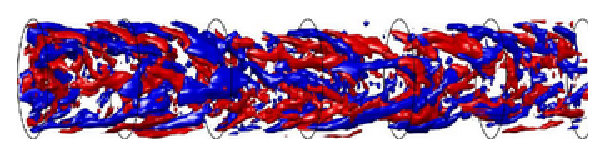
\includegraphics[width=0.90\textwidth]{vDoorne4}
\end{center}
\end{frame}


\begin{frame}{numerical challenges}
            \begin{block}{computation of turbulent solutions}
requires 3-dimensional volume discretization
\\
$\to$ integration of  $10^4$-$10^6$ coupled ordinary differential equations
            \end{block}

\bigskip

\begin{block}{challenging, but today possible}
J.F. Gibson
\HREF{http://channelflow.org/}{ChannelFlow.org}
\\
A. P. Willis
\HREF{http://www.openpipeflow.org/}{OpenPipeFlow.org}
            \end{block}
\end{frame}

\begin{frame}{example : pipe flow}
amazing data! amazing numerics!
\begin{center}
  \includegraphics[width=1.0\textwidth,clip=true]
                    {pipeSects}
\end{center}

\begin{itemize}
 \item here each instant of the flow $\approx$ 2.5\,MB
 \item videos of the flow $\approx$ GBs
\end{itemize}
\end{frame}

\begin{frame}{plane Couette : small computational cell, Eulerian velocity visualization}
\begin{center}
\includegraphics[width=0.5\textwidth]{statseSpProj3center}
\end{center}
next - the same solution, different visualization
\end{frame}

\begin{frame}{plane Couette isovorticity visualization}
\begin{center}
\includegraphics[width=1.0\textwidth]{ItGe09}
\end{center}
\end{frame}


\begin{frame}{part 2}
\begin{enumerate}
              \item
    \textcolor{gray}{\small
dynamical theory of turbulence
        }
              \item
    {\Large
\statesp
    }\textcolor{gray}{\small
              \item
space is time
              \item
dimension of the inertial manifold
                    }
            \end{enumerate}
\end{frame}


\section[dynamics in $\infty$ dimensions]
{dynamics in $\infty$ dimensions}

\begin{frame}{{\Large MUST} look at it in}
\bigskip
\hfill
{\Huge \statesp}
\vfill
E. Hopf 1948
\end{frame}

\begin{frame}{dynamical description of turbulence}
%	from {../chapter/dynsysII}

\begin{block}{\statesp}
a manifold $\pS \in \reals^{d}$ :
$d$ numbers determine the state of the system
\end{block}

\bigskip

\begin{block}{representative point }
$\ssp(t) \in \pS$
\\
a state of physical system at instant in time
\end{block}

\bigskip

\begin{block}{integrate the equations}
trajectory $\ssp(\zeit) = \flow{\zeit}{\xInit}$ =
representative point time $\zeit$ later
\end{block}
\end{frame}

\begin{frame}{representative point}
\begin{block}{example of a representative point (experimment)}
$\ssp(t) \in \pS$, $d= \infty$ \\
a state of turbulent pipe flow at instant in time
\end{block}

\bigskip

%%%%%%%%%%%%%%%%%%%%%%%%%%%%%%%%%%%%%%%%%%%%%%%%%%%%%%%%%%%%%%%%%%
%\hfill
%\begin{minipage}[c]{0.35\textwidth}
Stereoscopic Particle Image Velocimetry $\to$
3-$d$ velocity field over the entire pipe%
\footnote{\footnotesize
%"Stereoscopic PIV on transition in pipe flow",
Casimir W.H. van Doorne
(PhD thesis, Delft  2004)
%; 	{\tt www.ahd.tudelft.nl}
}

\bigskip

\begin{center}
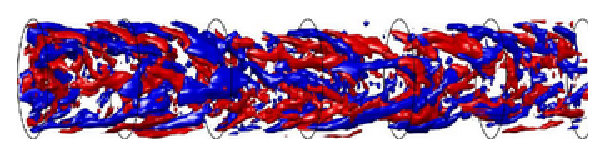
\includegraphics[width=0.90\textwidth]{vDoorne4}
\end{center}
\end{frame}

\begin{frame}{charting the state space of a turbulent flow}
John F Gibson (U New Hampshire)
\\
Jonathan Halcrow (Google)
\\
P. C.
\end{frame}

\begin{frame}{can visualize 61,506 dimensional \statesp\ of turbulent flow}
\begin{center}
\includegraphics[width=0.80\textwidth]{NCC1701b}
\end{center}
\eqva\ of turbulent plane Couette flow,
\\
their unstable manifolds, and
\\
myriad of turbulent videos mapped out as one happy family

\bigskip

\hfill   {\small
          for movies, please click through
            \textcolor{blue}{\href{http://ChaosBook.org/tutorials}
             {ChaosBook.org/tutorials}}
          }
\end{frame}

\begin{frame}{61,506 dimensional : Nagata's ``upper branch''}
\begin{center}
\includegraphics[width=0.48\textwidth]{UBmanifold4}
\end{center}
unstable manifold of an exact plane Couette equilibrium solution
\end{frame}

\begin{frame}{plane Couette state space $10^5 \to 3D$}
\begin{center}
\includegraphics[width=0.7\textwidth]{a1_14_g2}
\end{center}
\eqva, \po s, their (un)stable manifold

\hfill   shape the turbulence
\end{frame}

\begin{frame}{part 3}
\begin{enumerate}
              \item
    \textcolor{gray}{\small
dynamical theory of turbulence
              \item
\statesp
        }
              \item
    {\Large
space is time
    }\textcolor{gray}{\small
              \item
dimension of the inertial manifold
                    }
            \end{enumerate}
\end{frame}


\begin{frame}{(1+1) space-time dimensional ``Navier-Stokes''}
computationally not ready yet to explore the inertial manifold of
$(1+3)$\dmn\ turbulence - start instead with $(1+1)$\dmn\

\bigskip

\begin{block}{\KS\ time evolution equation}
\[
  u_t + u \triangledown u \,=\,
    {\color{red}-}\triangledown^2 u {\color{red}-\triangledown^4 u}
    \,,\qquad   x \in [-L/2,L/2]
    \,,
\]
\end{block}

\bigskip

describes spatially extended systems such as
\begin{itemize}
 \item flame fronts in combustion
 \item reaction-diffusion systems
 \item \ldots
\end{itemize}

\end{frame}

\section[KSe, $L=22$]{\KS, $L=22$, state space }

\begin{frame}{\KS\ on a large domain}
\begin{center}
  \includegraphics[width=0.9\textwidth,height=0.5\textheight,clip=true]
  {ksevol-fig} %{ks_largeL_cbar}
\end{center}

{\footnotesize
[horizontal] space $\ssp \in [0,L]$
\qquad
{[up]} time evolution
}

\begin{itemize}
\item turbulent behavior
\item simpler physical, mathematical and computational setting than Navier-Stokes
\end{itemize}
\end{frame}

\begin{frame}{
want : $(\conf,\zeit) \in (-\infty, \infty)\times (-\infty, \infty)$
             }

\bigskip

continuous symmetries : space, time translations
\medskip

\begin{center}
\includegraphics[width=1.1\textwidth]{spaceTime}
\end{center}
% \hfill \color{red}{(impossible without xxx)}
\end{frame}

\begin{frame}{
must have : 2D symbolic dynamics
$\in (-\infty, \infty)\times (-\infty, \infty)$
             }
\begin{center}
\includegraphics[width=0.8\textwidth]{recurrence}
\end{center}
% \hfill \color{red}{(impossible without xxx)}

\hfill Gutkin and Osipov (2015)
\end{frame}

\begin{frame}{compact space, infinite time cylinder}
\begin{center}
\includegraphics[width=0.9\textwidth]{cylinderTime}
\end{center}
% \hfill \color{red}{(impossible without xxx)}
so far : Navier-Stokes on compact spatial domains, all times
\end{frame}

\begin{frame}{compact space, infinite time \KS}

\begin{block}{in terms of discrete spatial Fourier modes}
$N$ ordinary differential equations (ODEs) in time
\[
\dot{\Fu}_k(\zeit) = ( q_k^2 - q_k^4 )\, \Fu_k(\zeit)
- i \frac{q_k}{2} \!\sum_{k'=0}^{N-1} \!\!\Fu_{k'}(\zeit) \Fu_{k-k'}(\zeit)
\,.
%\label{e-Fks}
\]
\end{block}
\end{frame}


\subsection{types of solutions}
\begin{frame}{evolution of \KS\ on small $L=22$ cell}
\begin{center}
  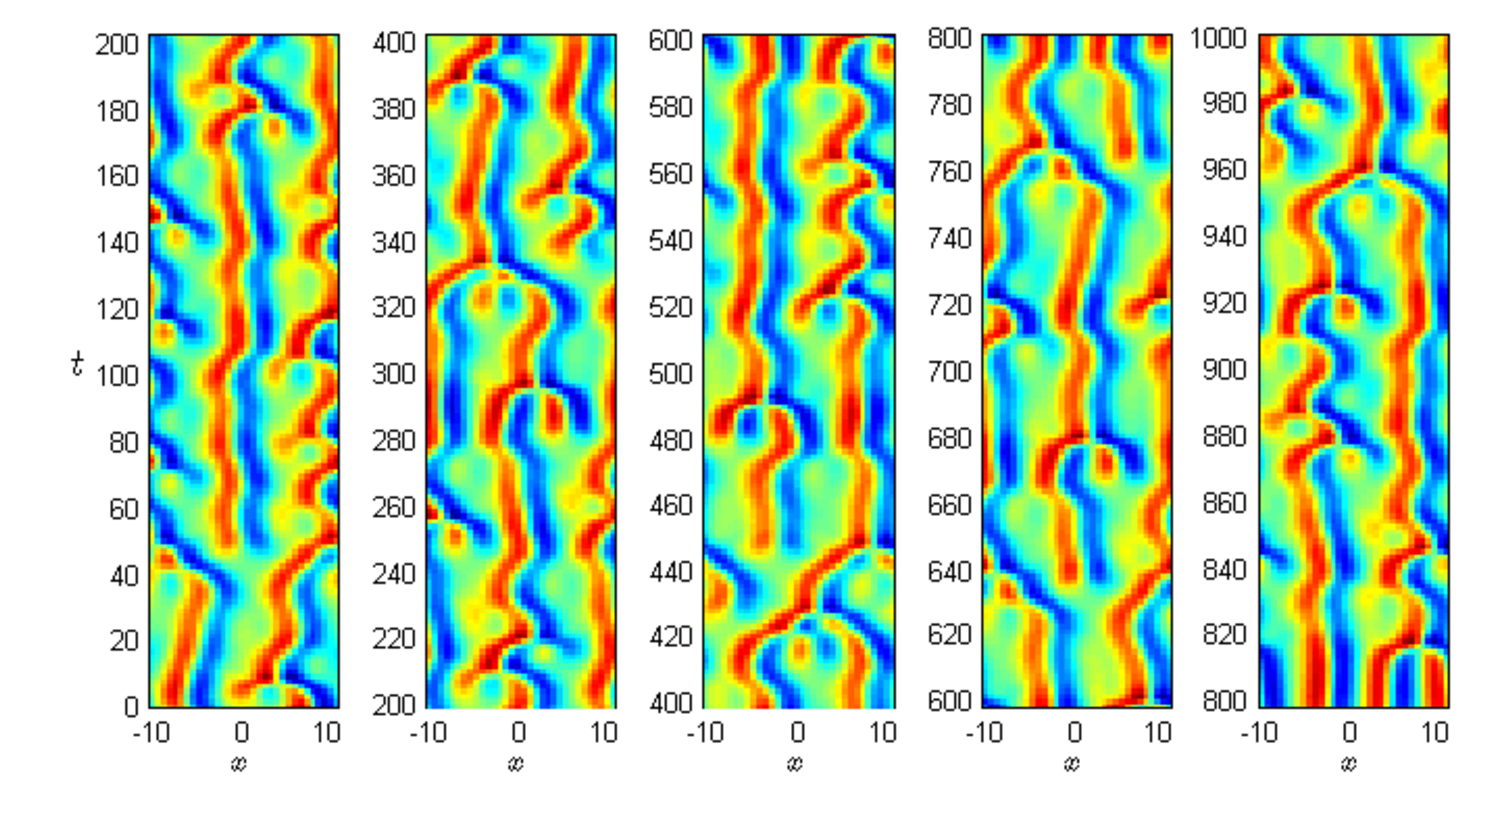
\includegraphics[width=0.9\textwidth,clip=true]{ks_L22_long_orbit}
\end{center}
horizontal: $x \in [-11,11]$
\\
vertical: time
\\
color: magnitude of $u(x,t)$
\end{frame}

\begin{frame}{a \rpo}
\begin{block}{full \statesp\ : many periods}
\begin{center}
\includegraphics[width=0.5\textwidth]{ks22torRPO1}
\end{center}
\end{block}
have computed: 60\,000 \po s
\end{frame}

\begin{frame}{can demonstrate shadowing etc}
\begin{center}
\includegraphics[width=0.6\textwidth]{ks22rpoT8072shad}
\end{center}
% \hfill \color{red}{(impossible without symmetry reduction)}
\end{frame}

\begin{frame}{\po s are dense in the attractor}
\begin{center}
\includegraphics[height=0.52\textwidth]{ksRecycled-ConfErgodic}
\includegraphics[width=0.545\textwidth]{ksPsectonPCA_POandErgodic}
\end{center}
\begin{itemize}
  \item {[left]} \textcolor{green}{turbulent trajectory} segment in [space$\times$time]
  \item \Poincare\ section, \textcolor{green}{turbulent trajectory} (natural measure)
  \item \textcolor{blue}{periodic points, from $479$ \po s}%
%\footnote{\footnotesize Budanur (PhD thesis 2015)}
\end{itemize}
\end{frame}

\begin{frame}{yes, but}
\begin{center}
{\huge is space time?}
\end{center}
\end{frame}

\begin{frame}{compact time, infinite space cylinder}
\begin{center}
\includegraphics[width=0.9\textwidth]{cylinderSpace}
\end{center}
% \hfill \color{red}{(impossible without xxx)}
\end{frame}

\begin{frame}{compact time, infinite space \KS}
\bea
    u_\zeit &=&  - u u_\conf
    -u_{\conf \conf}-u_{\conf \conf \conf \conf}\,,
    % \label{e-ks}
\continue
    u^{(0)} &\equiv& u \, , \quad
    u^{(1)} \equiv u_{\conf} \, , \quad
    u^{(2)} \equiv u_{\conf \conf} \, , \quad
    u^{(3)} \equiv u_{\conf \conf \conf}
                        \nonumber
\eea
\begin{block}{periodic boundary condition in time
              $u(\conf, \zeit) = u(\conf, \zeit + \period{})$}
evolve $u(\zeit, \conf)$ in $\conf$,
4 equations, 1st order in spatial
derivatives
\bea
    u^{(0)}_{\conf} &=& u^{(1)} \,,\quad
    u^{(1)}_{\conf}  =  u^{(2)} \,,\quad
    u^{(2)}_{\conf}  =  u^{(3)} \continue
    u^{(3)}_{\conf} &=& - u^{(0)}_{\zeit} - u^{(2)} - u^{(0)} u^{(1)}
                        \nonumber
\eea
\end{block}

\bigskip

initial values
$u( \conf_0, \zeit)$,
$u_{\conf}( \conf_0, \zeit)$,
$u_{\conf \conf}( \conf_0, \zeit)$,
$u_{\conf \conf \conf}( \conf_0, \zeit)$,
    \\
for all $\zeit \in [0, \period{})$ at a space point $\conf_0$
\end{frame}

\begin{frame}{a time-invariant \eqv, spatial \po}
\begin{center}
  \begin{minipage}[height=.45\textheight]{.45\textwidth}
    \centering \small{\texttt{(a)}}
    \includegraphics[width=\textwidth,height=.45\textheight]{MNGeq1time}
  \end{minipage}
  \begin{minipage}[height=.45\textheight]{.45\textwidth}
    \centering \small{\texttt{(b)}}
    \includegraphics[width=\textwidth,height=.45\textheight]{MNGeq1space}
  \end{minipage}
\end{center}
   %\caption{
  evolution of $\EQV{1}$ : (a) in time, (b) in space
   \\
   initial condition for the spatial integration is the time strip
   $u(\conf_0,\zeit)$, $\zeit = [0,\period{})$, where time period
   $\period{} =0$, spatial $x$ period is $L=22$.
   % }\label{fig:MNGeqva1spttmp}

\vfill\hfill        Michelson 1986
\end{frame}


\begin{frame}{chronotope}
\begin{bartlett}{
In literary theory and philosophy of language, the chronotope is how
configurations of time and space are represented in language and
discourse.
                }\bauthor{
\HREF{https://en.wikipedia.org/wiki/Chronotope}
{Wikipedia : Chronotope}
                }
\end{bartlett}

\bigskip
\bigskip
goes without saying : was done by a Soviet scientist first

\begin{itemize}
  \item Mikhail Mikhailovich Bakhtin (1937)
  \item Politi, Giacomelli, Lepri, Torcini (1996)
  \item Gutkin and Osipov (2015)
\end{itemize}
\end{frame}

\begin{frame}{chronotope : }

a finite $(1+D)$\dmn\ symbolic dynamics rectangle

\begin{center}
\includegraphics[width=0.8\textwidth]{recurrence}
\end{center}
\hfill \color{red}{make it doubly periodic}
\end{frame}

\begin{frame}{compact space and time chronotope}
\begin{center}
\includegraphics[width=0.9\textwidth]{torusSpTime}
\end{center}
% \hfill \color{red}{(impossible without xxx)}
\end{frame}

\begin{frame}{a spacetime \po}
\begin{center}
  \begin{minipage}[height=.40\textheight]{.35\textwidth}
    \centering \small{\texttt{(a)}}
    \includegraphics[width=\textwidth,height=.60\textheight]{MNGcomp32xint22}
  \end{minipage}
~~~~~~~~~
  \begin{minipage}[height=.40\textheight]{.35\textwidth}
    \centering \small{\texttt{(b)}}
    \includegraphics[width=\textwidth,height=.60\textheight]{MNGcomp64xint22}
  \end{minipage}
\end{center}
    (a) old : time evolution. (b) new : space evolution
    \\
    $x=[0,22]$,
       initial condition : time periodic line $t = [0,
   2\,T_{\PPO{10.2}})$
  %\label{fig:MNGcompxint2}
\end{frame}

\begin{frame}{each chronotope is a fixed point}
discretize $u_{n,m} = u(\conf_n,\zeit_m)$ over
$N M$ points of spatiotemporal periodic lattice $\conf_n = n \period{}/N$,
 $\zeit_m = m \period{}/M$, Fourier transform :
%\beq
%    \Fu_{k,m}^{(i)} = \frac{1}{M} \sum_{\ell = 0}^{M-1}
%    \Fu^{(i)}_{k,\ell} e^{i \omega_\ell \zeit_m}
%    \, , \quad
%    \Fu^{(i)}_{k,\ell} = \sum_{m=0}^{M-1}\Fu_{k,m}^{(i)}  e^{-i \omega_\ell \zeit_m}
%    \, , \quad
%    \mbox{where }
%    \omega_\ell = 2 \pi \ell / \period{} \, .
%\eeq
%
\[
\Fu_{k,\ell} \,=\,
  \frac{1}{NM} \sum^{N-1}_{n=0} \sum^{M-1}_{m=0}
  u_{n,m} \, e^{-i(q_k\conf_n + \omega_\ell \zeit_m)}
    \,,\quad
q_k = \frac{2 \pi k}{L}
    \,,\;
\omega_\ell = \frac{2 \pi \ell}{\period{}}
% \label{spattempFT}
\]
\KS\ is no more a PDE / ODE, but a fixed point problem of
determining all invariant unstable 2-tori
\[
\left[- i \omega_\ell - ( q_k^2 - q_k^4 ) \right]\Fu_{k,\ell}
+ i \frac{q_k}{2} \!\sum_{k'=0}^{N-1} \sum^{M-1}_{m'=0}\!\!
\Fu_{k',m'} \Fu_{k-k',m-m'}
    =
0
%\,.
%\label{e-FksSpattemp}
\]

\bigskip

Newton method for a $NM$\dmn\ fixed point :
\\ invert $1-J$,
\\ where $J$ is the
2-torus Jacobian matrix, yet to be elucidated
\end{frame}

\begin{frame}{dynamical Zeta function for a field theory}
  \begin{columns}
  \column{0.42\textwidth}
\begin{block}{$\infty$ of spacetime tilings}
\[
Z(s) \approx
\sum_{p} \frac{e^{-A_p s}}
              {\left|\det(1-J_p)\right|}
\]
tori / plane tilings
\\
each of area $A_p = L_p T_p$
\end{block}
  \column{0.53\textwidth}
\begin{block}{trace formula  for a field theory}
\includegraphics[width=0.9\textwidth,clip=true]{pde2}%
\end{block}
  \end{columns}
\end{frame}

%\section[dimension of the inertial manifold]
%{dimension of the inertial manifold}

\begin{frame}{part 4}
\begin{enumerate}
              \item
    \textcolor{gray}{\small
dynamical theory of turbulence
              \item
\statesp
              \item
space is time
    }
              \item
    {\Large
dimension of the inertial manifold
                    }
            \end{enumerate}
\end{frame}

\begin{frame}{turbulence, and its physical dimension}

you say : "but the $MN$ spacetime discretization of a PDE is HUUUUUUUUGE !"

    \begin{minipage}[b]{0.30\textwidth}
\begin{block}{inertial
 manifold
}
\end{block}
    \end{minipage}
~~~~~~
    \begin{minipage}[b]{0.60\textwidth}
\begin{center}
\includegraphics[width=0.8\textwidth]{inertialMan}
\end{center}
    \end{minipage}

\medskip
strange attractor stuffed into
a \textcolor{red}{\Large finite-dimensional} body bag
\end{frame}

\begin{frame}{linearized deterministic flow}

%%%%%%%%%%%%%%%%%%%%%%%%%%%%%%%%%%%%%%%%%%%%%%%%%
 \begin{center}
  \setlength{\unitlength}{0.65\textwidth}
  %% \unitlength = units used in the Picture Environment
  \begin{picture}(1,0.48527529)%
    \put(0,0){\includegraphics[width=\unitlength]{covariant1}}%
    \put(0.82300289,0.05462827){\color[rgb]{0,0,0}\rotatebox{0.03306771}{\makebox(0,0)[lb]{\smash{$\ssp_n$}}}}%
    \put(0.25001124,0.20377481){\color[rgb]{0,0,0}\rotatebox{0.03306771}{\makebox(0,0)[lb]{\smash{$\ssp_{n+1}$}}}}%
    \put(0.39195273,0.41066662){\color[rgb]{0,0,0}\rotatebox{0.03306771}{\makebox(0,0)[lb]{\smash{$\jMps_n$}}}}%
    \put(0.89193475,0.41023002){\color[rgb]{0,0,0}\rotatebox{0.03306771}{\makebox(0,0)[lb]{\smash{$\vel_n$}}}}%
    \put(0.03306474,0.40112261){\color[rgb]{0,0,0}\rotatebox{0.03306771}{\makebox(0,0)[lb]{\smash{$\vel_{n+1}$}}}}%
  \end{picture}%
 \end{center}
%%%%%%%%%%%%%%%%%%%%%%%%%%%%%%%%%%%%%%%%%%%%%%%%%
\[
\ssp_{n+1} + \orbitDist_{n+1}= f(\ssp_n) + \jMps_n \, \orbitDist_n
      \,, \quad
\jMps_{ij} = \partial f_i / \partial \ssp_j
\]

\medskip

in one time step a linearized neighborhood of $\ssp_n$ is
\begin{enumerate}
	\item[(1)] advected by the flow
	\item[(2)]
transported by the \jacobianM\ $\jMps_n$ into a
neighborhood given by the $\jMps$
eigenvalues and eigenvectors
\end{enumerate}
\end{frame}

\begin{frame}{(2) Floquet vectors}
\setlength{\unitlength}{0.40\textwidth}
\begin{center}
              \begin{minipage}[b]{0.40\textwidth}
  \begin{picture}(1,0.66867674)%
    \put(0,0){\includegraphics[width=\unitlength]{covariantPO}}%
    \put(0.74435424,0.20540854){\color[rgb]{0,0,0}\rotatebox{0.0313674}{\makebox(0,0)[lb]{\smash{$\jEigvec[1]$}}}}%
    \put(0.64622163,0.40053847){\color[rgb]{0,0,0}\rotatebox{0.0313674}{\makebox(0,0)[lb]{\smash{$\jEigvec[2]$}}}}%
    \put(0.89791873,0.38658395){\color[rgb]{0,0,0}\rotatebox{0.0313674}{\makebox(0,0)[lb]{\smash{$\ssp(0)$}}}}%
    \put(0.12764619,0.54392048){\color[rgb]{0,0,0}\rotatebox{0.0313674}{\makebox(0,0)[lb]{\smash{$\ssp(\tau)$}}}}%
    \put(0.4259836,0.61739585){\color[rgb]{0,0,0}\rotatebox{0.0313674}{\makebox(0,0)[lb]{\smash{$\jMps^\tau$}}}}%
    \put(0.35028678,0.33942992){\color[rgb]{0,0,0}\rotatebox{0.0313674}{\makebox(0,0)[lb]{\smash{$\jEigvec[1]$}}}}%
    \put(0.05904285,0.32095124){\color[rgb]{0,0,0}\rotatebox{0.0313674}{\makebox(0,0)[lb]{\smash{$\jEigvec[2]$}}}}%
  \end{picture}% % \label{f:covariantPO}
              \end{minipage}
\end{center}

\bigskip

a parallelepiped spanned by a pair of Floquet eigenvectors (`covariant
vectors') transported along the orbit
\end{frame}

\begin{frame}{dimension of the inertial manifold}

\bigskip

\begin{itemize}
  \item Floquet modes separate into \entangled\ vs. \transient
\end{itemize}
\end{frame}

\begin{frame}{(1) \KS\ physical dimension \\ two large cells : it scales!}
\begin{center}
\includegraphics[width=1.0\textwidth]{YaTaGiChRa08fig4}
\end{center}

now double \# Fourier modes :
\\
all new ones go to the \transient\ spectrum

\vfill\hfill
%\footnote{\footnotesize
Yang et al (2009)
%}
\end{frame}

\begin{frame}{summary : dynamical zeta function for a field theory}
\begin{block}{"\po s" are now spacetime tilings}
\[
Z(s) \approx
\sum_{p} \frac{e^{-A_p s}}
              {\left|\det(1-J_p)\right|}
\]
tori / spacetime tilings :
each of area $A_p = L_p T_p$
\end{block}
\begin{block}{symbolic dynamics : $(1+D)$\dmn}
essential to encoded shadowing

\hfill Gutkin and Osipov (2015)
\end{block}

\vfill
at this time : it is till but a dream
\end{frame}


\begin{frame}{what is next for Bogomolny? take the course!}
\begin{center}
\includegraphics[width=0.65\textwidth]{posterCB2cover}
\end{center}
\vfill
student raves : \\
...$10^6$ times harder than any other online course...
\end{frame}



\end{document}
